\documentclass[notitlepage]{report}
\usepackage{graphicx}
\usepackage{listings}
\graphicspath{{../pdf/}{/Users/nat/uni/cs342-labs/cw2}}
\usepackage{titling}
\usepackage{titlesec}
\titleformat{\chapter}
  {\normalfont\large\bfseries}{\thechapter}{1em}{}
\titlespacing*{\chapter}{0pt}{3.5ex plus 1ex minus .2ex}{2.3ex plus .2ex}

\titleformat{\section}
  {\normalfont\bfseries}{\thesection}{1em}{}
\titlespacing*{\section}{0pt}{3.5ex plus 1ex minus .2ex}{2.3ex plus .2ex}

\titleformat{\subsection}
  {\normalfont\bfseries}{\thesubsection}{1em}{}
\titlespacing*{\subsection}{0pt}{3.5ex plus 1ex minus .2ex}{2.3ex plus .2ex}

\usepackage{etoolbox}
\makeatletter
\patchcmd{\chapter}{\if@openright\cleardoublepage\else\clearpage\fi}{}{}{}
\makeatother

\pretitle{\begin{center}\Huge\bfseries}
\posttitle{\par\end{center}\vskip 0.5em}
\preauthor{\begin{center}\Large}
\postauthor{\end{center}}
\predate{\par\large\centering}
\postdate{\par}

\title{CS342 Machine Learning\\Assignment 2}
\author{Nathan Frend u1319248}
\date{\today}
\begin{document}

\maketitle

\begin{abstract}
This project aims to identify and classify fish using images taken aboard fishing ships as a part of The Nature Conservancy's online competition on kaggle. This report will discuss the three feature engineering techniques used: Histogram of Gradients,  Principal Component Analysis and Geometric transformations. The two models being used are Multi-Layer Perceptrons and Convolutional Neural Networks with the former also using the three feature engineering techniques as input. An analysis of each model and its performance will be given at the end of the report.
\end{abstract}

\tableofcontents

\chapter{Data Exploration \& Feature Engineering}
Of the training data supplied the majority of images are 1280 by 720 pixels. Some of the images are larger than this but are truncated to 1280 by 720 when loaded so as to keep the data consistent. This size of image would result in 921600 pixels which translates to the same number of features that need to be considered. This is a large amount of features to be considered when constructing a model so in order to reduce computation time the images will be reduced in size and blurred to reduce the number of pixels and therefore features in each image. The images will be reduced to 640 by 360 pixels which reduces the number of features to 1/4 of what it was before.

\section{Principal Component Analysis}
PCA is a feature engineering technique that focuses on the variation and patterns within the dataset. In the context of this project PCA may help for the model to realise parts of the image showing the boat don't help to identify the class of fish. It does this by removing features that are common amongst the dataset and focusing on the features with maximum variance. This should theoretically also help to speed up the model as there are less features to compute. 

Using Sklearn's implementation of PCA the parameter n\_components was tweaked so as to result in getting around 100 features after PCA has been carried out. A value of 0.7 worked well to reach this number. 

\section{Geometric transformations}
Geometric transformations are a useful feature engineering method to generate a larger data set from the already existing one. By translating or rotating an image from the data set, a new image can be created. If this is applied to the whole data set then the size of that set can double for each time a new set is created by rotating or translating. There is a risk of cropping the fish out of the generated new image however if the crop is quite small the risk of this should be relatively low and should cause less of a negative than the gain of using a larger data set.
\begin{figure}[h!]
\centering
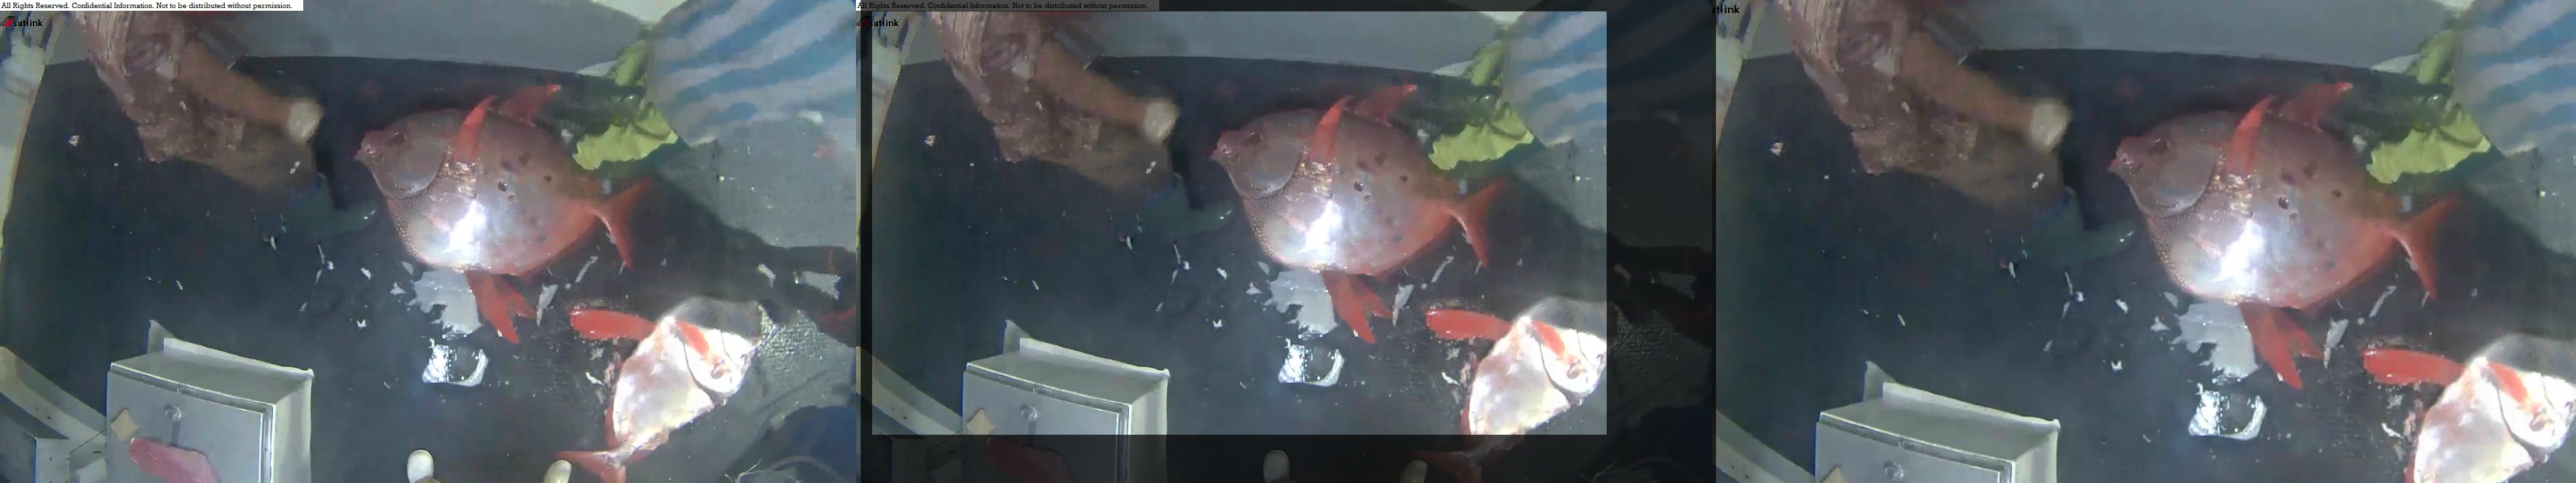
\includegraphics[scale=0.08]{example}
\caption{How a new image can be generated from a crop of the original}
\end{figure}

Applying this method to the training data set of this project should result in more accurate readings. To accomplish this, rather than compute using the whole image, the image used will instead be a crop of the original image. This cropped image will be smaller than the original but only by a few pixels. This is similar to thinking of the crop being a mask or a window over the top of the image that can be move around so as to generate new images from the original.

\section{Histogram of Gradients}
HOG is another feature engineering technique that also tries to reduce the number of features of an image by focusing only on useful features and removing features that aren't as useful. This is accomplished by first calculating the gradient images. These gradient images show where there's a sharp change in intensity in the image which would signify an edge. The edges are important as it means an outline of important parts within the picture are still easily distinguishable but smaller due to the irrelevant data in between being removed.

Next the image will be broken up into parts with each part representing a group of gradients. By using these parts we can further reduce the number of features in the image. Since each part can be thought of an averaged value of the whole, HOG also gives the advantage of being less sensitive to noise within images.

\chapter{Machine Learning: Models Artificial Neural Networks and Deep Learning}
\section{Multi-Layer Perceptron using raw pixel values as inputs}
The first implementation of this model was quite inaccurate as the original version used the raw image data from the whole image. The raw image would first be read in by opencv and then resized so as to be constrained to a specific grid size so as to keep all the training vectors the same size. This resizing would result in the image being resampled by setting the \textit{interpolation} parameter to \textbf{INTER\_AREA} when using the \textit{cv2.resize()} method.
\section{Multi-Layer Perceptron using feature engineering techniques as inputs}
\subsection{HOG \& PCA}
The first model I constructed using feature engineering techniques used a combination of HOG and PCA. In order to do this first each image had it's HOG computed and then the resulting vector was truncated so as to keep the number of features consistent. The vectors would then be stored in an array which would then be passed to Sklearn's PCA method. These features engineering techniques helped to improve the algorithm greatly.
\subsection{Geometric Transformations \& PCA}
The second model used a combination of translating the images to generate new images and then PCA to reduce the number of features. The use of HOG as well would have meant a huge increase in the time taken to train the model due to the large increase in the size of the data set caused by the translating.
\section{Convolutional Neural Network using raw pixel values as inputs}
\chapter{Progression Graph \& Conclusion}

\end{document}